\section{Introduction}

With the recent rise in sales in the smartphone/PDA market
and the recent launch of several tablet form-factor devices (Tablet PCs, Apple iPad, Amazon's Kindle), users increasingly use medium sized touch screens. These screens offer
more screen space than a traditional phone, and can arguably be more
effective in text-input tasks. Due to increased size and weight,
however, these devices require specific postures for the users to be
able to input text. Therefore, text entry on such devices continues to be a difficult problem.

As mentioned above, the tablet form-factor introduces two major problems for the user. 

Firstly, the larger form-factor makes it hard to type while not seated. Since a tablet is portable, it is an ideal device for use while mobile. By this we mean situations when the user is actually moving between different places, but mostly stationary. Commuters standing in a train are a good example of users who would benefit from using a computing device while standing, walking or sitting and briefly holding their device.
\begin{figure}
    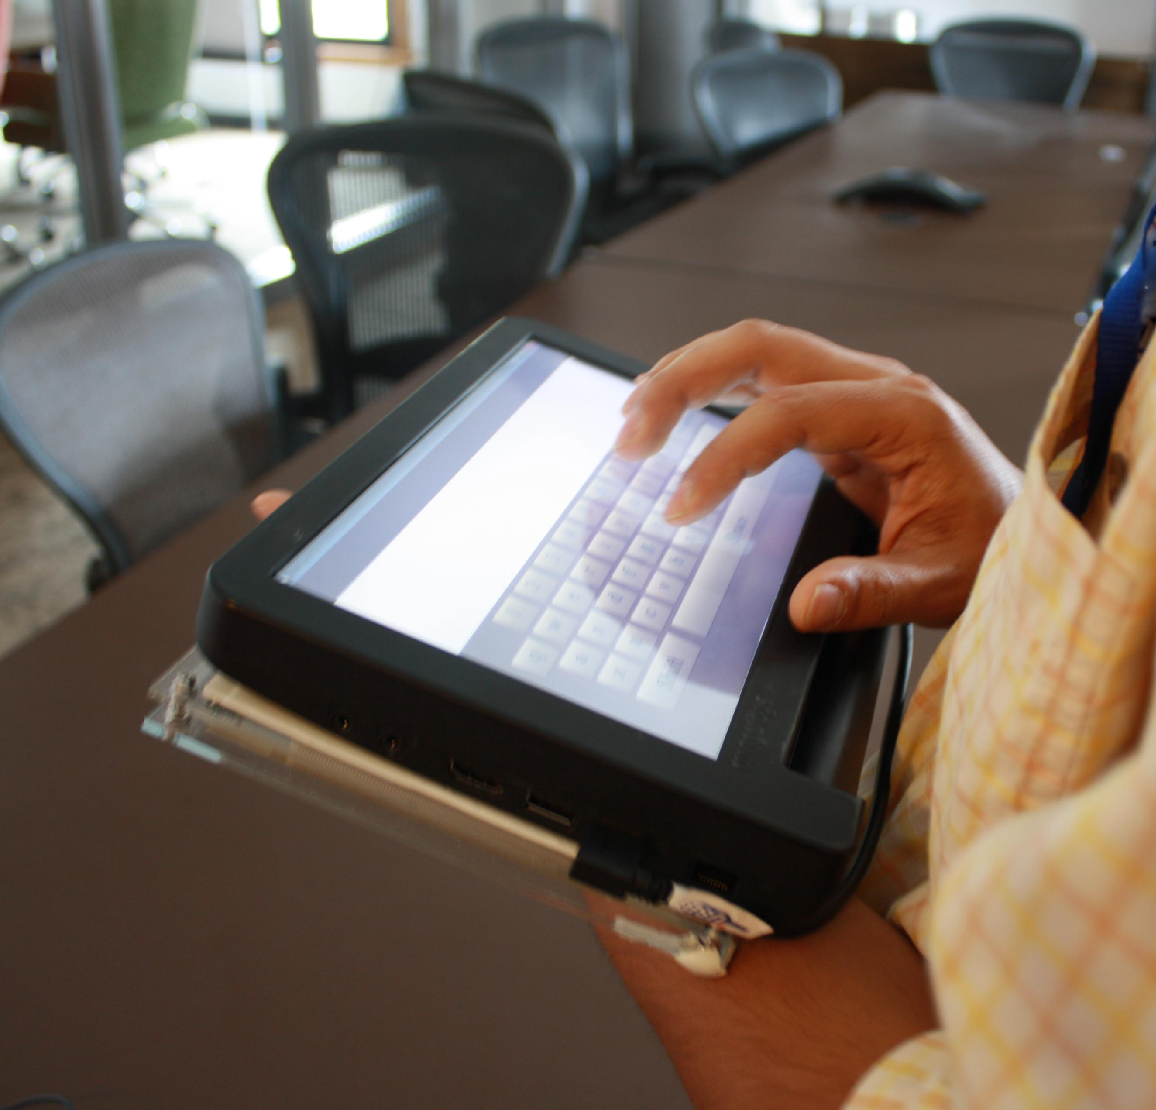
\includegraphics[scale=0.35]{Figures/device_hold.pdf} 
  	\caption{A user holding a tablet form-factor device and trying to enter text. It can be seen how this is unstable and unnatural.}
    \label{fig:device_hold}
\end{figure}
Unlike a mobile phone, however, a larger (e.g. 7+ inches wide)  keyboard (soft or otherwise) does not work well with two thumbs because of the relatively large distance that the thumbs must travel to reach the appropriate keys. The weight of the device compounds the problem of typing by straining the hands to support the device while making precise movements to position the thumbs over the proper keys. While standing, many users resort to a different pose, in which one arm supports the device while the other hand types with a single finger (Figure~\ref{fig:device_hold}). 

The second problem with tablet form-factor is that direct touch or pen input cause the issue of occlusion. Previous work suggests that such scenarios involve contortions of fingers and hands to achieve a configuration that allows for reading the screen while entering text. \cite{Vogel}

At the same time, there has recently been a push in the industry for devices with "backside" input, in which the device has a touch input device or keyboard on the opposite side of the main display. Notion Ink's Adam PC has a backside trackpad [1]. Samsung, Toshiba and Sony have also been making effort towards backside touch input \todo{citations}. As manufacturers start to include backside input in their devices, we have an opportunity to take advantage of this new input modality to improve the users speed, accuracy and comfort while entering text on their tablet form-factor devices. A "natural" method of holding such a device is to have hands on both the sides with fingers wrapped around on the back. \cite{Vogel} (Figure~\ref{fig:natural})

We believe that back-of-device interactions offer solution to both the problems mentioned above because the fingers naturally rest on the back of the device while holding it, thereby relieving the common problem of trying to hold a device with one hand while tapping with the other. (Figure~\ref{fig:device_hold}) Moreover, keeping the finger input on the back keeps the fingers from getting in the way of viewing the information on the screen. A concrete scenario to consider is when the user is mobile but still visually focused, but occasionally losing focus while entering text (for example while commuting on a train).  With a QWERTY keyboard, users have to orient themselves again after each lapse. Such scenarios can benefit from mechanisms that don't require the user to reorient themselves when they lose focus.  Scenarios in which the user is only intermittently focused, such as when they are walking, require mechanisms that help the user memorize certain set patterns and configurations of fingers, that they could later replicate even without looking at the interface. 

In this paper we present two text-input mechanisms that can be tested on devices with back-of-device touch input. The goal is to provide mechanisms that could allow users to enter text on devices with tablet form-factor and back-of-device touch input in a way that eliminates the problems of occlusion of screen space inherent to touch and pen input, and uses the established effectiveness of vertical movements on back-of-device touch input \cite{Wobbrock} by giving freedom of movement to multiple fingers. Previous studies \cite{RearType},\cite{LucidTouch} have tried to investigate a similar design space, but there is lack of systematic understanding of back-of-device text-input in the absence of additional hardware like hover sensing (LucidTouch) and discrete physical keys (RearType). 

In this paper we present a novel text-input mechanism that could be
tested on devices with back-of-device touch input, and examine QWERTY
layouts on both the front and back of the device for comparison. The
goal is to provide mechanisms that could allow users to enter text on
devices with larger screens and back-of-device touch input in a way
that eliminates the problems of occlusion of screen space inherent to
touch and pen input, and uses the established effectiveness of
vertical movements on back-of-device touch input \todo{cite Wobbrock}
by giving freedom of movement to multiple fingers.  Our work stands in
contrast to other recent work which requires additional hardware, such
as hover sensing \todo{cite LucidTouch} or discreet physical keys
\cite{RearType}.

We have designed a chording-based touch input mechanism specifically for devices with a back-of-device touch input.  This mechanism shows promise in the scenarios described above.  Figure~\ref{fig:natural} illustrates that entering text on the back of the device results in a more natural, comfortable and stable pose than the commonly adopted pose shown in Figure~\ref{fig:device_hold}.  We designed the mechanism to use large, relatively inaccurate finger movements as the building
block for chords.  This allows the user to exploit proprioceptive feedback (e.g. the feedback from in the nervous system of the hands that signals the relative positions of the fingers to one another) to
increase their speed and accuracy by reducing or eliminating the visual feedback required to enter text. We also designed a backside-QWERTY mechanism that allows users to use multiple fingers to manipulate multiple cursors, thereby entering text. Details on both the mechanisms can be found later in the paper.

\begin{figure*}
    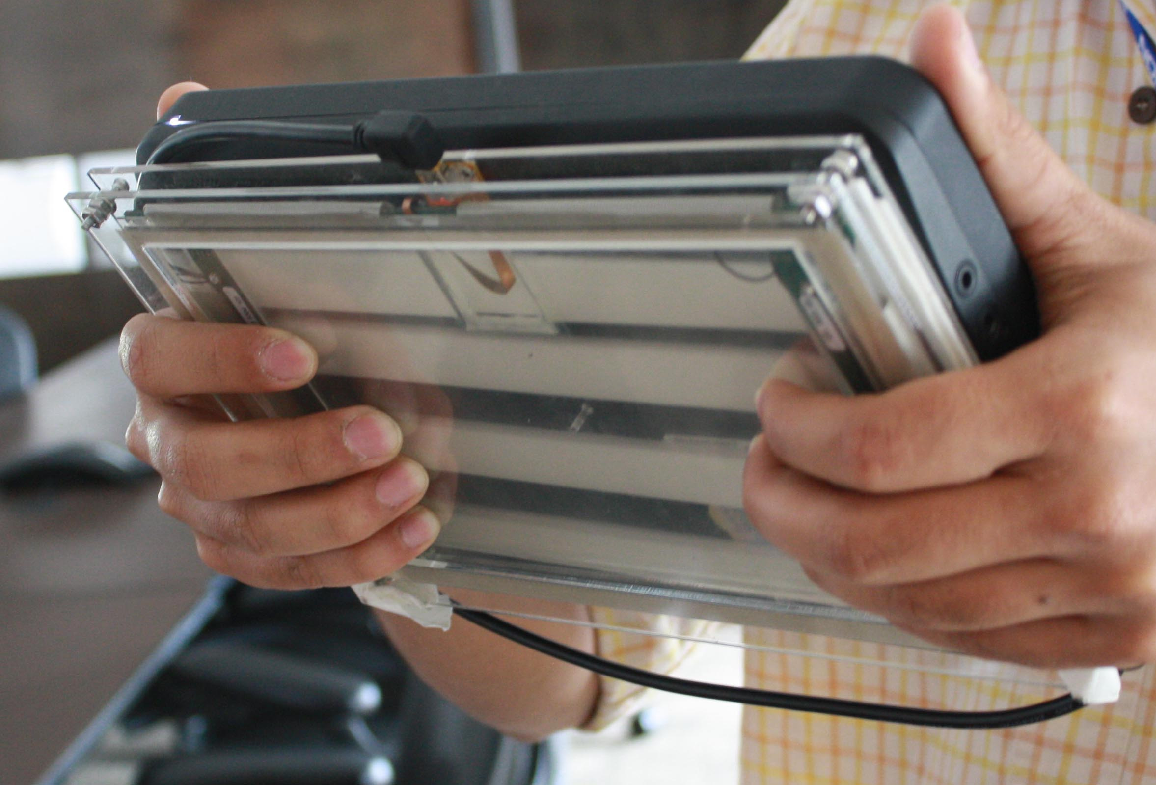
\includegraphics[scale=0.43]{Figures/natural1.pdf} 
     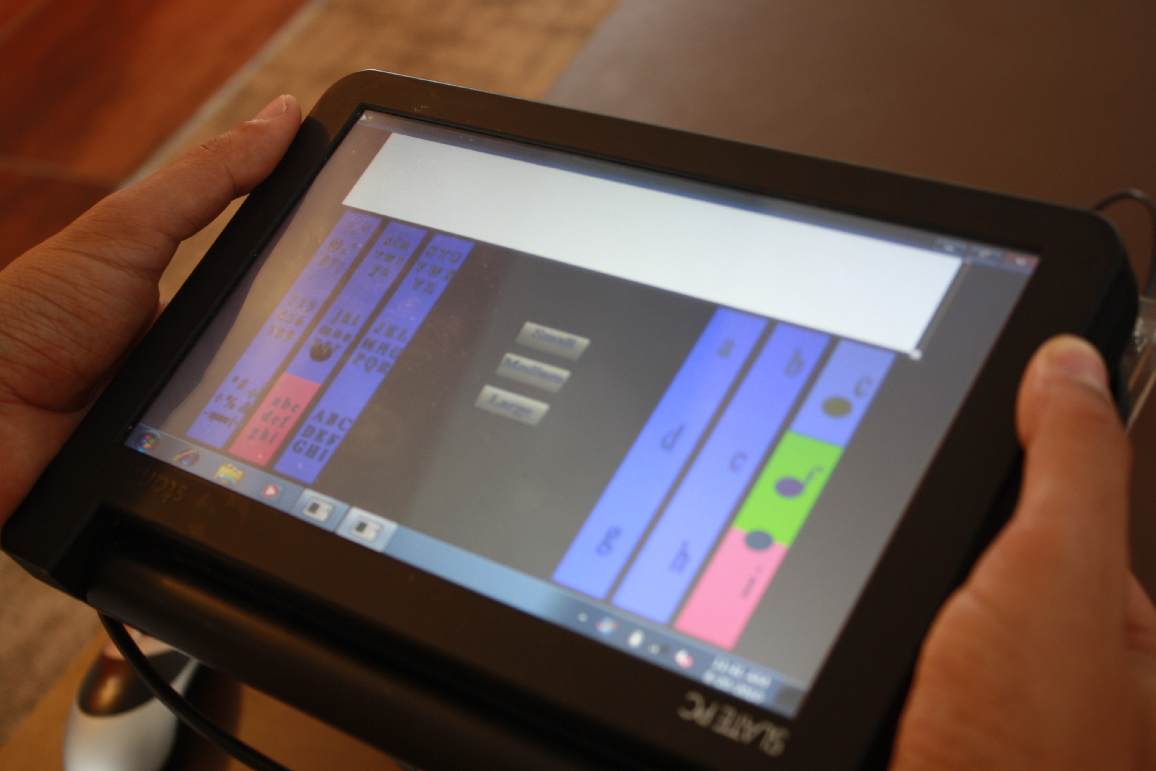
\includegraphics[scale=0.43]{Figures/natural2.pdf} 
     \caption{A user holding a mobile device with medium-sized touch
       screen in a natural and stable posture. The user is able to see
       his finger positions on the screen on the front. The figure
       also shows our hardware prototype with a multitouch screen on
       the rear of a Slate PC.}
        \label{fig:natural}
\end{figure*}

In the paper we detail our initial quantitative and qualitative investigation of these new mechanisms. However, just like in the case of other exploratory works \cite{RearType} our focus for this phase of experimentation was to determine if users find such input mechanisms usable or frustrating. There can also be additional concerns with use of back-of-device touch input, like minimized grip stability. In view of such issues it was necessary to investigate the user perception around back-of-device text-input. To capture that we use the NASA Task Load Index (TLX) and present an analysis of the reported user experience. Using a hardware prototype with a multitouch input on both the back and the front of the device, we compare the performance of the novel chording mechanism and a backside QWERTY with a standard soft QWERTY keyboard on the front or the back of the device in a controlled, 36-user study. We found that with less than an hour of training, users of the backside-QWERTY were able to type 3/4th as fast as soft-QWERTY. Also the chording mechanism turned out to be the most efficient in terms of KSPC (Keystrokes per Character)